\chapter{Protocol Design}
\label{chap:protocoldesign}

In the state of the art, there are different protocols constructed over \ac{IEEE} 802.15.4, like ZigBee, WirelessHART, 6LoWPAN, etc. Some
are prepared for low consumption, but almost none of them is focused on localization. To cover this necessity, as an alternative, 
\ac{LPL} and \ac{OLP} \cite{LPLandOLP} protocols were proposed in the department. These protocols are based on 
\ac{IEEE} 802.15.4 and are specifically designed for low consumption localization. In the next sections a brief overview will be given, 
for a deeper view, please consult \cite{LPLandOLP}.

\section{\ac{LPL} and \ac{OLP}}

\ac{LPL} and \ac{OLP} \cite{LPLandOLP}, are two protocols designed for localization, in particular localization using \ac{RSSI} 
values. These values give an idea of the received signal strength in the device, knowing that the higher this value,
the nearer the device. \ac{RSSI} have the big advantage that its value is already included in all packets a device receives. There
is hence no need for special hardware or data to be prepared or obtained like in other methods (Ultra Wide Band e.g.). But \ac{RSSI} 
values have a big problem for localization, its dispersion is very big, making the localization resolution (in some cases up to 
many meters \cite{fingerprint}) inappropriate for some applications. 

However, this resolution problem can be solved. One solution is using localization techniques like ``fingerprint 
technique'' \cite{fingerprint} to improve the resolution. Another option is, taking more than one \ac{RSSI} value to obtain a more stable 
result. This technique has one big challenge, the more values are taken, the higher the energy consumption. Without a good approach, 
the \ac{MN} would need to listen to the channel most of the time waiting to receive packets from \ac{AN} to obtain \ac{RSSI} values. 
This way a lot of energy would be wasted just doing nothing during what is called idle listening. \ac{LPL} and \ac{OLP} propose two different 
approaches to solve this.

Another important aspect in localization is which kind of node calculates the position. Three different alternatives can be obtained.

\begin{itemize}
 \item \textbf{Centralized.} A central computer receives the \ac{RSSI} values from all \acp{AN} in the network and calculates the positions of 
the \acp{MN}. The advantage is that the computer can use complicate algorithms to obtain better results, but this method 
charges the network with a lot of traffic, specially if the \ac{MN} needs to know its position after calculation.
 \item \textbf{Distributed-A.} The \ac{AN} gets the \ac{RSSI} values directly from the packet sent by the \ac{MN}, and this \ac{AN}
calculates directly the \ac{MN} position. This method does not charge the network like the centralized approach but the resolution 
is not that good. It is important to note that each \ac{MN} has a ``selected \ac{AN}''. This \ac{AN} is the one in charge to 
calculate \ac{MN} position and the one the \ac{MN} communicates with and through. This \ac{AN} is usually the closest one to 
the \ac{MN}.
 \item \textbf{Distributed-M.} In this mode, the \ac{MN} is who calculates directly its position from \ac{RSSI} values obtained from \acp{AN}.
The problem is that \acp{MN} cannot use powerful localization algorithms. This solution almost does not charge the network.
\end{itemize}

The protocols \ac{LPL} and \ac{OLP} are going to use different phases for different behaviors, and these phases will be repeated cyclically. To 
make this possible, all nodes have to start the phases at the same time. This makes necessary a good synchronization among all nodes.
Nodes will get the synchronization information from their parents (do not forget that a tree topology is used) using an active or a passive synchronization. 
To get a graphical explanation check Figure \ref{fig:synchronization}.

\begin{itemize}
 \item \textbf{Passive Synchronization.} The parent starts the process sending a packet (R1) to \ac{MAC} Layer to be transmitted, this packet is
created at the time-stamp Tx1, and includes this time, the time until the next phase start (TF) and info about this phase. Due to random time in 
\ac{CSMA/CA} process and other processing times, R1 is not transmitted immediately but in Tx2. When the packet is transmitted, \ac{MAC} Layer informs
the application layer and this creates another packet (R2) including the new time-stamp Tx2. At the child, 2 packets will be received, R1 and 
R2 in times Rx1 and Rx2 respectively. Calculation of next phase start, from the child's point of view (TZ), is accomplished like in (\ref{mat:pasivesync}).

\begin{equation}
  TZ = TF - (Rx2 - Rx1) - (Tx2 - Tx1)
  \label{mat:pasivesync}
\end{equation}

\begin{figure}[ht]
 \begin{center}
  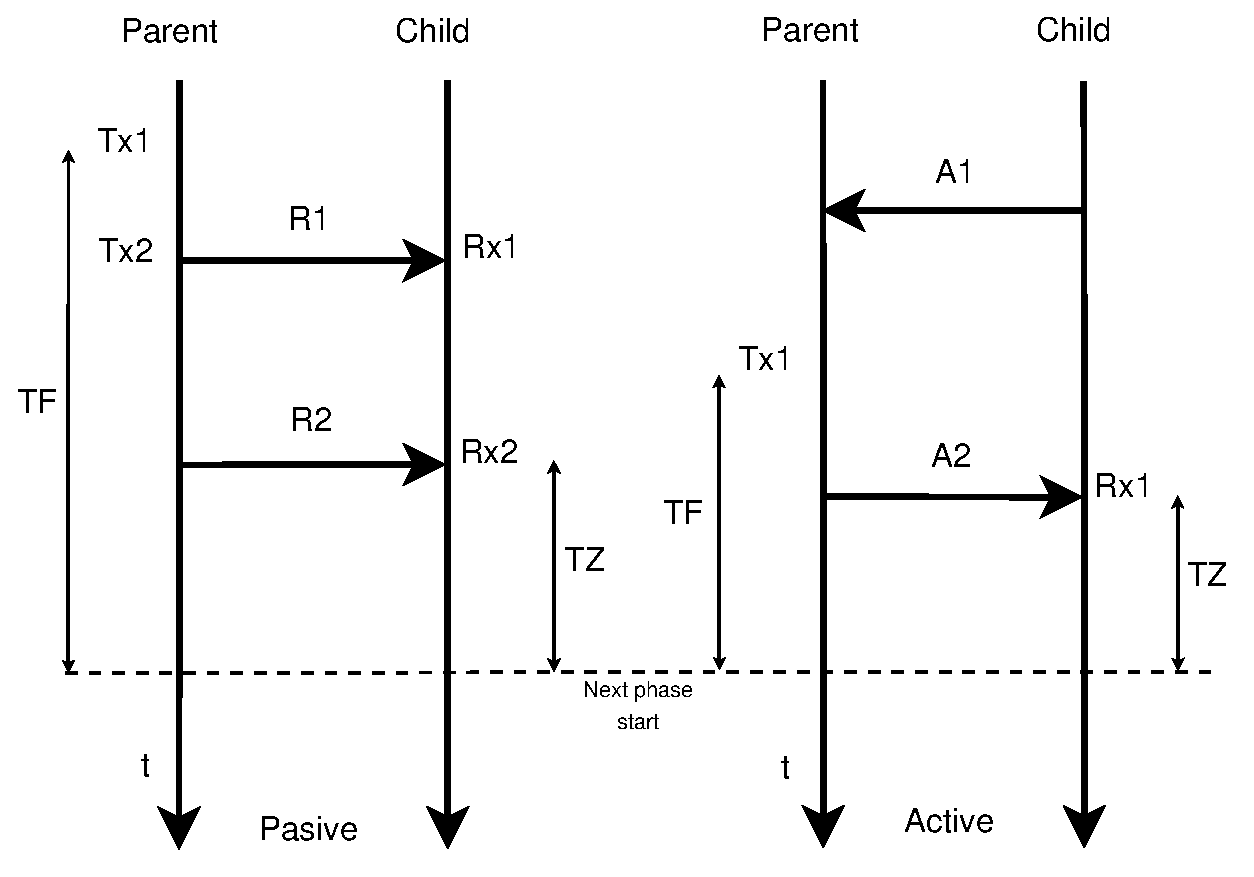
\includegraphics[width=0.6\textwidth]{synchronization.eps}
 \end{center}
 \caption{Passive and Active Synchronization \cite{LPLandOLP}}
 \label{fig:synchronization}
\end{figure}
 
 \item \textbf{Active Synchronization.} In the active synchronization, the child starts the process sending a synchronization request (A1).
Then the parent answers with packet A2, which contains the time until the start of the next phase (TF). The child can calculate this time
with the equation in (\ref{mat:activesync}).

\begin{equation}
  TZ = TF - C
 \label{mat:activesync}
\end{equation}

The C parameter in (\ref{mat:activesync}), represents an estimation of all the processing times and random times from \ac{CSMA/CA}. For that reason 
this method is not so exact like the passive one, but it does not need two packets.
\end{itemize}

In the following subsections, both protocols \ac{LPL} and \ac {OLP} are going to be explained.

\subsection{\acl{LPL}}

To reduce the idle listening, and thus the energy consumption, this protocol proposes that \acp{MN} do not listen to the \acp{AN}. Instead, the
\acp{MN} are the ones who transmit and the \acp{AN} the ones who listen and transmit this information to the central computer. This protocol is 
divided into three phases which can be appreciated in Figure \ref{fig:LPL}.

\begin{figure}[ht]
 \begin{center}
  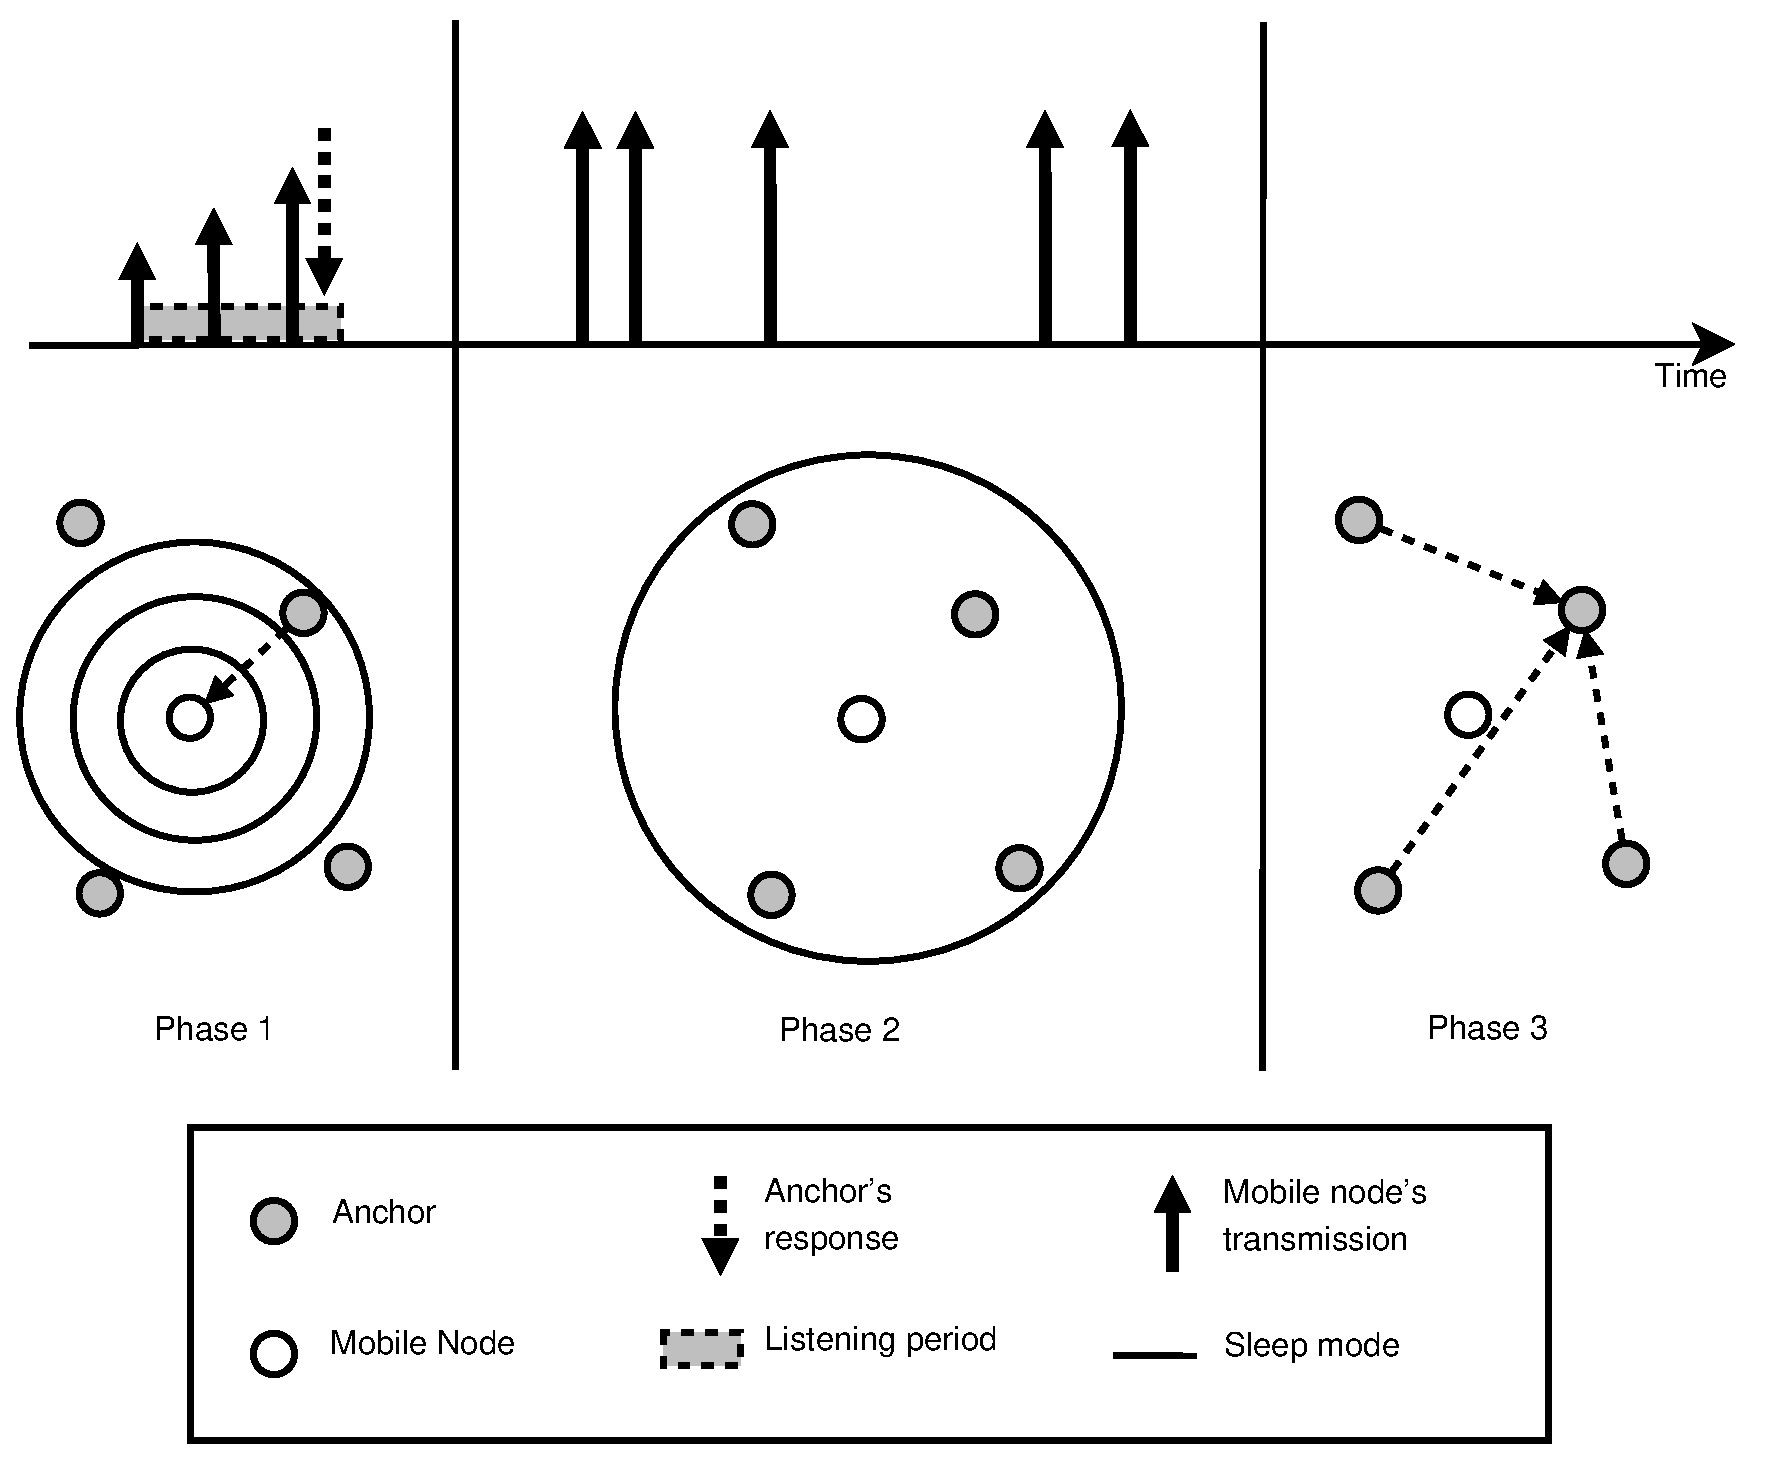
\includegraphics[width=0.7\textwidth]{LPL.eps}
 \end{center}
 \caption{LPL Phases \cite{LPLandOLP}}
 \label{fig:LPL}
\end{figure}

\begin{itemize}
 \item \textbf{Phase 1:} In this phase, \ac{MN} selects a random time to broadcast a synchronization request, starting with the minimum power,
and increasing this power until it receives an answer from an \ac{AN}. This will be the selected \ac{AN}, and the answer will contain information
about the phase times. This process makes sure that only the nearest \acp{AN} answer to the synchronization request. In the next phase 1, if 
the \ac{MN} needs to know its position, it asks its selected \ac{AN} about this information, and if not, it just synchronizes.
 \item \textbf{Phase 2:} In phase 2, the \ac{MN} broadcasts several packets in random times to minimize the collisions. Each time the node is not
transmitting, it goes to sleep. This way \acp{MN} are awake only when they transmit, eliminating the idle listening. The \acp{AN} that
received this broadcasts, store the read \ac{RSSI} values and the selected \ac{AN} address.
 \item \textbf{Phase 3:} During this phase, the \acp{MN} sleep and the \acp{AN} send the measured \ac{RSSI} values to the selected \ac{AN}. 
This \ac{AN} will calculate the \ac{MN} position in Distributed-A case or send the data to a central computer in Centralized case. In this phase, both 
synchronization among the \acp{AN} and the network configuration take place.

This protocol, has some disadvantages that make it not suitable for all conditions:

\begin{itemize}
 \item Hidden Terminal Problem. This is a serious problem not only because it could cause big idle listening in phase 2, but also because the number
of collisions could be high and the packets would have been sent for nothing, wasting a lot of energy. In phase 1, it could also 
happen that, if two \acp{MN} transmit at the same time, the selected \ac{AN} might not be the closest one to the \ac{MN} but one with a bad connection.
 \item High \ac{MN} number. If the number of \acp{MN} is high, phase 2 is going to be full of collisions and thus, the idle listening will be
high. This problem would be worse due to the hidden terminal problem.
 \item Selected \ac{AN} selection. In phase 1, if many \acp{AN} are close to the \ac{MN}, all of them are going to try to answer causing collisions. Also, 
when the \acp{AN} are not close to the \ac{MN}, a lot of energy is wasted in the \ac{MN} trying to detect gradually the selected \ac{AN}.
\end{itemize}


\end{itemize}


\subsection{\acl{OLP}}

In the case of \ac{OLP} protocol and unlike \ac{LPL}, the \ac{MN} is the one who listens. This protocol is also divided in 3 phases, 2 of 
them can be appreciated in Figure \ref{fig:OLP}.

\begin{figure}[ht]
 \begin{center}
  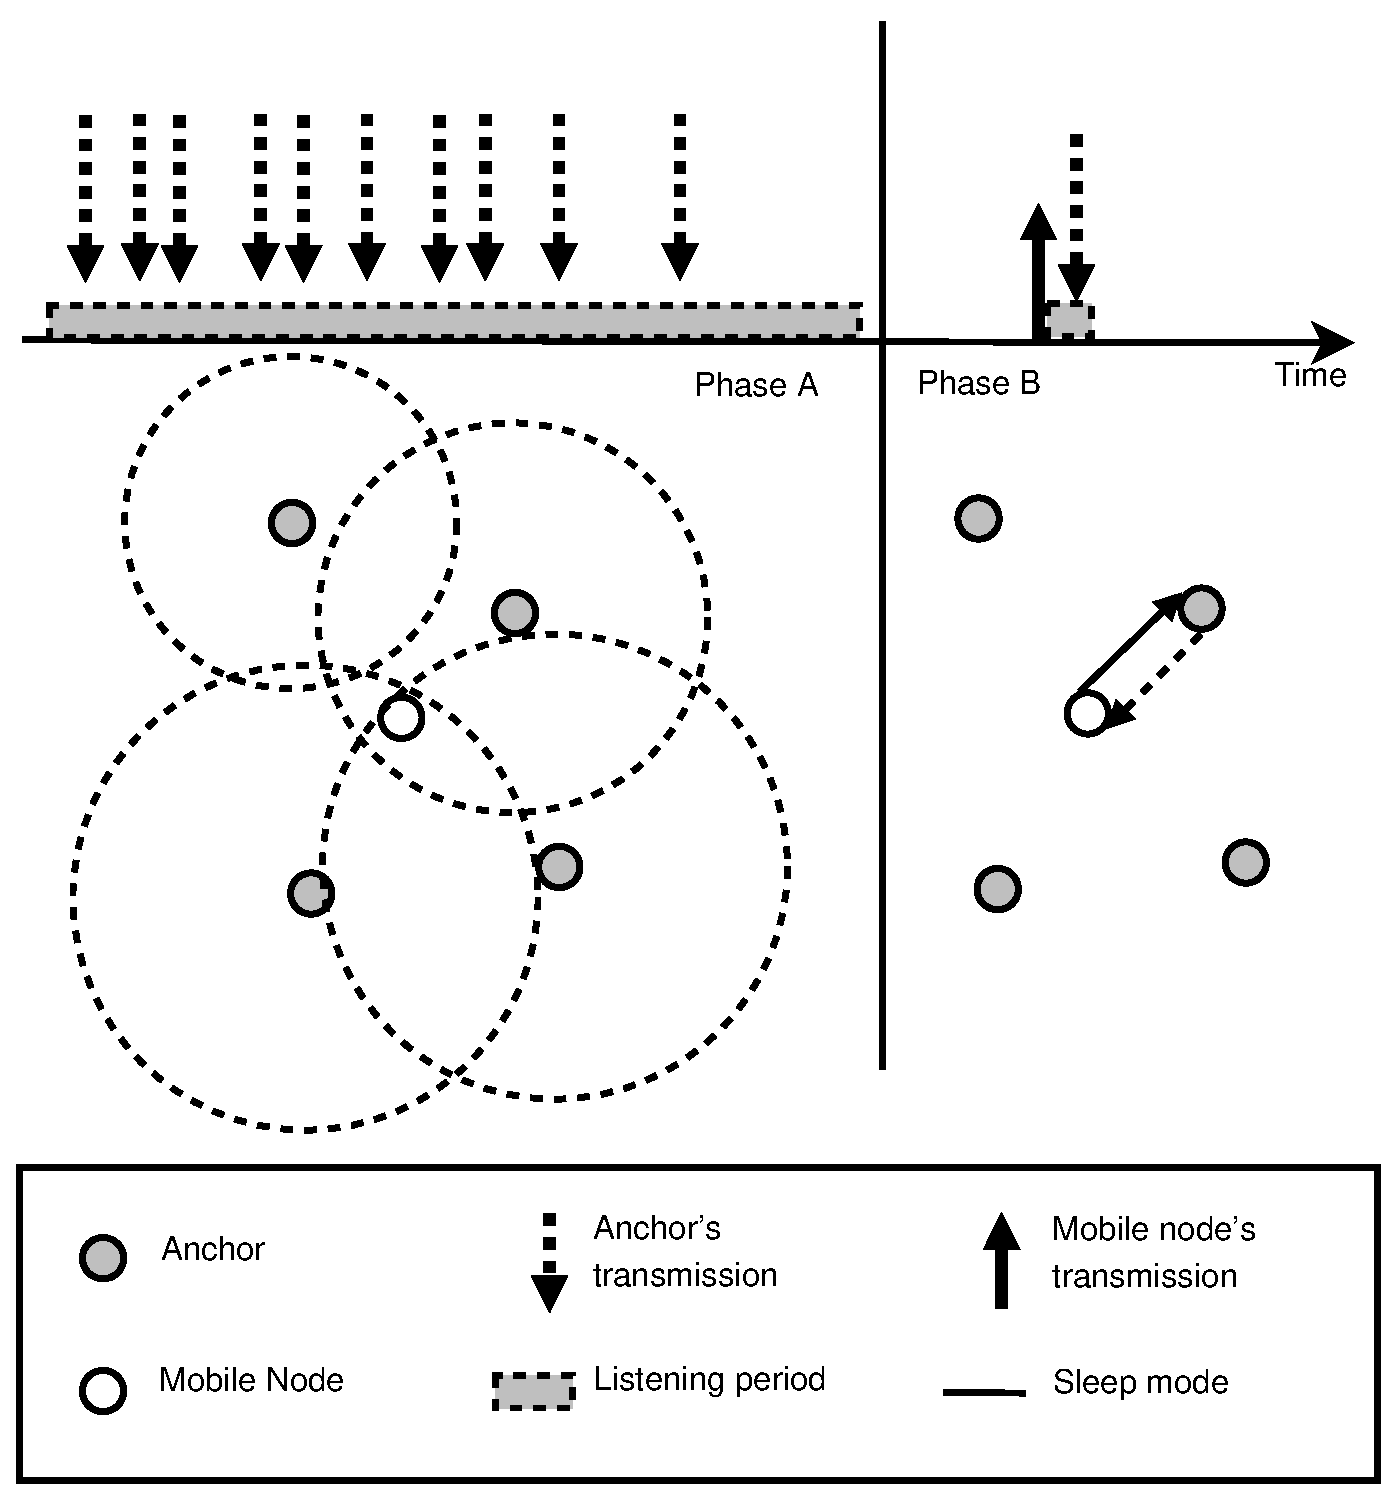
\includegraphics[width=0.55\textwidth]{OLP.eps}
 \end{center}
 \caption{OLP Phases \cite{LPLandOLP}}
 \label{fig:OLP}
\end{figure}

\begin{itemize}
 \item \textbf{Phase A:} In this phase, and thanks to the synchronization among \acp{AN}, the inter-arrival time is reduced, decreasing so the
idle listening. This packets also contains synchronization information for the \ac{MN}. In this phase \ac{RSSI} values are received and stored
by the \ac{MN}. Then it goes to sleep.
 \item \textbf{Phase B:} In this phase and in Distributed-M mode, the \ac{MN} will use easy localization algorithms together with all the obtained
\ac{RSSI} values to calculate its position. In case of Distributed-A or Centralized mode, the \ac{MN} will send a report to the selected \ac{AN}, taken 
from the highest \ac{RSSI} value, with all the stored \ac{RSSI} values in Phase A. The selected \ac{AN} will answer with an \ac{ACK}. In the following
phase B, the \ac{MN} will ask the selected \ac{AN} about its position in case it needs it.
 \item \textbf{Phase C:} Like in \ac{LPL} this Phase is reserved for communication among \acp{AN} and network configuration.
\end{itemize}

\ac{OLP} has also some problems:

\begin{itemize}
 \item Synchronization. In this protocol, a really good \acp{AN} synchronization is needed to make the idle listening in phase 1 from the 
\acp{MN} as low as possible. This is not easy, specially with a tree structure where the synchronization error will be increased and 
propagated through the tree.
 \item \ac{MN} listens too much. The \ac{MN} is listening during long periods of time where all the \acp{AN} are transmitting, some times it
could even happen that the \ac{MN} it is not at a reachable distance from the \ac{AN} that is transmitting, listening in this moment just 
for nothing.
 \item Hidden Terminal Problem. If the \acp{AN} are not good synchronized to avoid this problem, the \acp{MN} would get many invalid 
packets, what means a waste of energy. If the number of \acp{MN} is big, then in phase 2 we could have many collision problems.
 \item Temporal \ac{RSSI} Correlation. As the \ac{RSSI} values are very correlated in near times \cite{RSSIcorrelated}, receiving all 
the packets so close in time would not contribute to have a better and more stable \ac{RSSI} measurement.
\end{itemize}
 

\section{High Configurable Protocol proposal}
\label{sec:ProtocolDescription}

From the previous section and according to the results in \cite{LPLandOLP}:
\begin{quote}
``LPL consumes lower energy than OLP when many RSSI samples are required from many ANs. On the other hand,
OLP becomes more energy efficient than LPL when there are several MNs and few RSSI samples are needed.''\cite{LPLandOLP}
\end{quote}

From this could be extracted that depending on the application, and the network load, it could be better that some nodes could have a 
configuration where their main action is listening and others could have a configuration where their main action is broadcasting. This 
configuration should be variable depending on the current network situation and the necessities of the node. From this arises the necessity
of a High Configurable Protocol with different node configurations.

As it was seen, \ac{OLP} and \ac{LPL} localization protocols, are based on \ac{RSSI} values. This work is also based on localization using 
\ac{RSSI} values. Anyhow, this simulation work proposes a framework for the protocol and does not try to locate any node, it concentrates
in the communication aspects and defines a base for the protocol to be developed further in future works.


\subsection{Node Configurations}

From the Table \ref{tab:wsn_applications} (page~\pageref{tab:wsn_applications}) where different applications for \ac{WSN} where stated and the
previous quotation, it is possible to extract these four different node configurations.

\begin{itemize}
 \item \textbf{Mode 1.} This is the normal configuration, when the \ac{MN} does not have any special need. A \ac{MN} with this configuration,
will listen to the \acp{AN} and then send the selected \ac{AN} a packet with the measurements. This is equivalent to having just \ac{OLP}. This
configuration supports the Centralized and Distributed-A working modes.

 \item \textbf{Mode 2.} This configuration mode is similar to mode 1, but in this case it is prepared to work only with Distributed-M working mode.
From time to time, if it is needed, the \ac{MN} could send the estimated positions to its selected \ac{AN}.

 \item \textbf{Mode 3.} This configuration, also called \ac{VIP} mode, is used when the node's battery is in a critical situation.
This configuration is similar to \ac{LPL} where the \ac{MN} broadcasts and the \acp{AN} receive the packets and send them to a coordinator that
will be able to estimate \ac{MN} position. When it is needed, a way for the \ac{MN} to request its position is provided, this will be explained 
later. The number of sent broadcasts is defined with the parameter \textit{NumberOfBroadcasts}.

 \item \textbf{Mode 4.} Unlike the previous configuration, this configuration is for nodes without battery problems, and with a high accuracy
need. This configuration is a mix of mode 1 and 3, the \ac{MN} listens to the \acp{AN} broadcasts but also they broadcast their
own packets to be measured by the \acp{AN}. All this information together is sent to a coordinator that will estimate \ac{MN} position.
This Mode as well as Mode 3 loads the network so much and will be used just when strictly needed. The number of sent broadcasts is also defined with 
the parameter \textit{NumberOfBroadcasts}.
\end{itemize}

This is just a brief description of the different configurations. As the protocol is yet to be explained, a full behavior description from 
every configuration will be done later together with the protocol description.

\subsection{Protocol Description}

From the previous section, it is obtained that this protocol, needs at least three different phases to work. One of the phases is a Sync 
Phase, where the \acp{AN} will transmit broadcasts and the \acp{MN} will listen to get \ac{RSSI} values and synchronize. Another needed 
phase is a phase where \acp{AN} and \acp{MN} could communicate among them. And the last required phase, is the one where the \acp{AN} could 
communicate with each other to and from the coordinator.

\acp{MN} configured with mode 3, are nodes with critical battery. These nodes must not waste energy, and this means their idle listening must be
as low as possible. As this nodes will not waste time listening and will just transmit broadcasts, it could be interesting reserving a phase
just for them, where their transmissions will not interfere with the ones from the rest of the \acp{MN}. This phase will be called \ac{VIP} 
Phase. It is clear, that the number of \ac{VIP} \acp{MN} cannot be too big, if so, their exclusivity will not be anymore exclusive.
This phase should not last too long, as there are still many other \acp{MN} to transmit and the phases collection would become too long.
The phase for communication among \acp{MN} and \acp{AN} will be named Report Phase, and here is where Mode 4 \acp{MN} can make 
their broadcasts and where communication among \acp{MN} and \acp{AN} can take place.

The main purpose of the phase where \acp{AN} communicate with each other, is to transmit information between the coordinator, also called sink, and 
the \acp{MN}. That is the reason why this phase will be called ComSink Phase. This phase should be the biggest one, as all traffic from 
the \acp{MN} should reach the sink and come back, and all \acp{AN} must transmit their own \acp{MN} information and route the one coming from
their sons or parents. As the traffic in this phase will be high, it could be useful to separate up-links traffic and down-links traffic. 
ComSink Phase will be divided in ComSink Phase 1 (up-links) and ComSink Phase 2 (down-links).

As it was said, \ac{RSSI} values are very correlated in time instants that are next to each other \cite{RSSIcorrelated}. That is why it could 
be favorable to distribute the Sync Phase to get better \ac{RSSI} samples. The whole period is formed by Sync Phase, Report Phase, \ac{VIP}
Phase, ComSink Phase 1 and ComSink Phase 2. If Report Phase and \ac{VIP} Phase are considered together in the phases distribution, Sync 
Phase can be divided into three phases separated in time: Sync Phase 1, Sync Phase 2 and Sync Phase 3. These sync phases will be intercalated 
between the other phases.

This phase collection will be repeated in time, being the period every phases collection repe\-ti\-tion. For a better understanding of this 
phase division, check Figure \ref{fig:ProtocolPhases}. This Figure will be explained in detail later.

\begin{figure}[ht]
 \begin{center}
  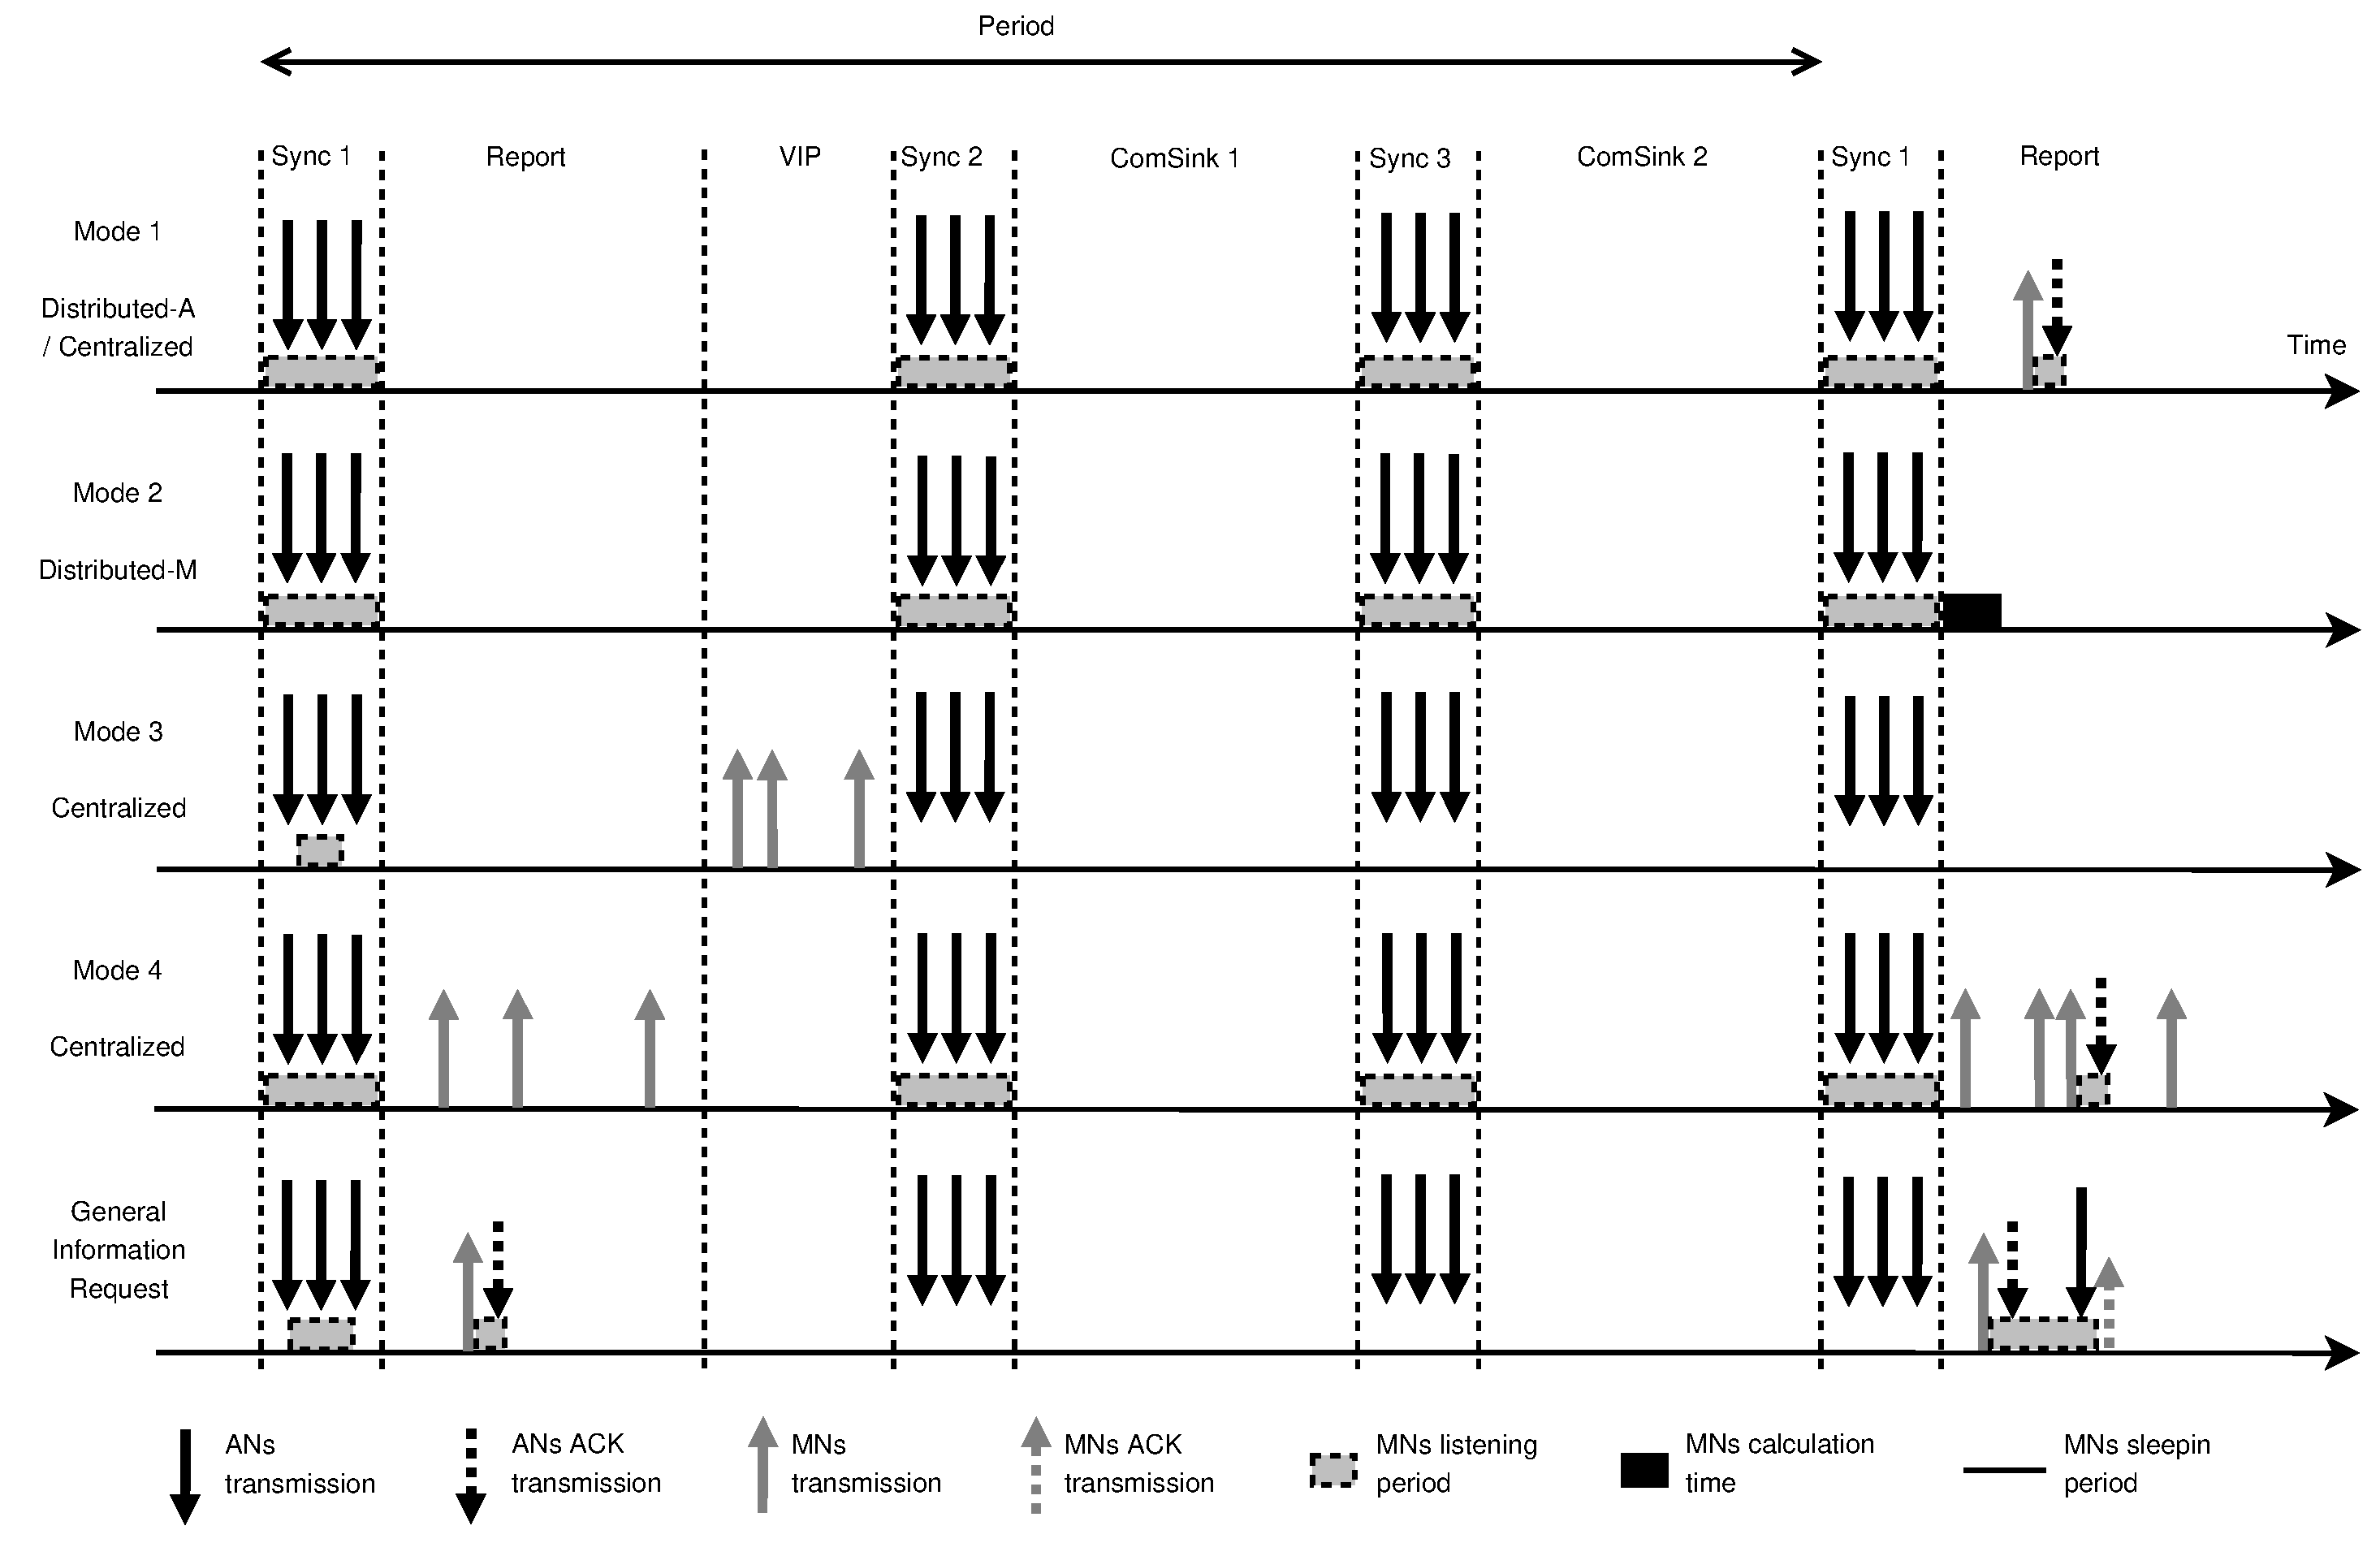
\includegraphics[width=1\textwidth]{ProtocolPhases.eps}
 \end{center}
 \caption{High Configurable Protocol Phases \cite{mipaper}}
 \label{fig:ProtocolPhases}
\end{figure}

The Figure \ref{fig:ProtocolPhases} is divided into 5 sections, one per Configuration Mode and the last one for explaining the General Information
Request. To understand properly how the protocol works, these sections have to be explained in detail:

\begin{itemize}
 \item \textbf{Mode 1.} \acp{MN} listen during the Sync Phases to the \acp{AN} broadcasts, and read the \ac{RSSI} values and send them
to their selected \ac{AN} during the Report Phase. This is obtained from the highest measured \ac{RSSI}. The selected \ac{AN} answers with an \ac{ACK} 
to the \ac{MN}. \acp{MN} sleep during the \ac{VIP}, ComSink 1 and ComSink 2 Phases as well as during Report Phase when no transmitting. 
\acp{AN} will communicate among them during ComSink 1 phase (up-links) and during ComSink 2 phase (down-links). This aspect is common for all the 
modes, that is why it will be commented only in this one. Whenever the \ac{MN} must communicate something to the selected \ac{AN} and no report 
is going to be sent during the period, it can schedule an extra report during the Report Phase. This extra report behavior is the same as the report 
where the \ac{RSSI} values are sent.
 
 \item \textbf{Mode 2.} Like in Mode 1, \acp{MN} listen during the Sync Phases to the \acp{AN} broadcasts, and read the \ac{RSSI} values. Instead
of sending them and due to the fact that packets also contain information of \acp{AN} localization, it is the \ac{MN} who calculates its own position 
and saves it. From time to time, these positions information will be sent to the coordinator via the selected \ac{AN} during the Report Phase. The 
selected \ac{AN} will answer with an \ac{ACK} to the \ac{MN} which go to sleep. \ac{MN} sleeps, like Mode 1, during \ac{VIP}, ComSink 1 and ComSink 2 
Phases as well as during Report Phase when no transmitting.

 \item \textbf{Mode 3.} Unlike Mode 1 and 2, Mode 3 does not listen during the Sync Phases but sleeps.Once in a while, Mode 3 will not sleep during a 
Sync Phase and will listen just for a couple of packets (not the whole phase) to resynchronize. During the \ac{VIP} Phase, the \ac{MN} will broadcast
some packets that will be listened by the \acp{AN} in the surrounding. This \acp{AN} will send the \ac{RSSI} information to the coordinator during the 
ComSink 1 phase, and this will calculate the \ac{MN} position. As Mode 1, \acp{MN} in Mode 3 could schedule an extra report during Report Phase to
communicate something to the selected \ac{AN}. Mode 3 \acp{MN} sleep during Sync, Report, ComSink 1 and ComSink 2 phases as well as during \ac{VIP} phase
when not transmitting. Whenever a \ac{MN} sends an extra report, during that period it will not send the broadcasts during \ac{VIP} Phase, this is to 
save energy, as with the extra report it will send already \ac{RSSI} information to the selected \ac{AN}.

 \item \textbf{Mode 4.} This is a combination of Modes 1 and 3. On one hand, the \acp{MN} listen during Sync Phases to get \ac{RSSI} values and send them
to their selected \ac{AN} during Report Phase waiting for an \ac{ACK}. But on the other hand, they broadcast also their own packets during the Report Phase.
This broadcasted \ac{RSSI} values are sent by all \acp{AN} to the coordinator who with all these values and the values reported by the \ac{MN} through the 
selected \ac{AN}, calculates the \ac{MN} position. As for Mode 1, whenever a \ac{MN} wants to send something, it can schedule an extra report. This node sleeps
during \ac{VIP}, ComSink 1 and ComSink 2 phases as well as during Report Phase when no transmitting.

 \item \textbf{General Information Request.} What happens if a \ac{MN} wants to know its position? or if it wants to change its configuration, how does it
warn the coordinator? Thanks to the General Information Request, this can be solved. During Report Phase and using a report or extra report, the \ac{MN}
will activate in this packet an ASK flag to notify the selected \ac{AN} that some data (the requested info is given in this packet) will be requested 
during next period in Report Phase, than the \ac{AN} acknowledges the packet like always. During the next Report Phase, the \ac{MN} will generate an extra
report in case there is no scheduled one and will activate the Request flag to notify the \ac{AN} that it wants the data asked the previous period about. As soon
as the \ac{MN} receives the \ac{ACK} from the selected \ac{AN}, a timer starts. If during this timer no packet from the selected \ac{AN} is received, the whole
process is canceled and it could be tried again later. If during this timer the \ac{MN} receives a packet from the selected \ac{AN}, the \ac{MN} sends an
\ac{ACK} to the \ac{AN} and the process is finished. The \ac{AN} will send a packet to the \ac{MN} even to indicate that it has no information available.
Doing so, idle listening in \ac{MN} is avoided.

This process must be done from time to time even if the node does not have any change or requirement, because if the coordinator wants to communicate with a
\ac{MN}, which would be sleeping all the time, this is the only way to reach it.
\end{itemize}

Like for \ac{LPL}, all packets sent (report and broadcasts), are sent in a random time using \ac{CSMA/CA} to minimize collisions.

Previously, it was just defined the standard behavior of the different configurations, but to really extract a high configuration of the protocol, some 
parameters must be taken into account.

\begin{itemize}
 \item \textbf{activePhases -} These are the periods where the \acp{MN} are active with their standard behavior (already commented).
 \item \textbf{inactivePhases -} These are the periods where the \acp{MN} are sleeping during all the phases.
 \item \textbf{offsetPhases -} These are the periods to leave inactive before the first active period comes.
 \item \textbf{offsetSyncPhases -} This is the number of Sync Phases during the first active period where the \acp{MN} do not listen, it will be explained 
better with an example.
 \item \textbf{reportPhases -} One period out of \textit{reportPhases}, the \ac{MN} will send an extra report in case this period does not have already one
scheduled. This happens even if the period is an inactive one.
 \item \textbf{askFrequency -} Every \textit{askFrequency} number of extra reports, these will have the ASK flag activated.
 \item \textbf{offsetReportPhases -} These are the periods to leave before the first extra report is scheduled.
\end{itemize}
 
As an example to explain these parameters check Figure \ref{fig:parametersphases}, where the parameters take the following values: 

\begin{quote}
 \textit{activePhases} = 2 | \textit{inactivePhases} = 2 | \textit{offsetPhases} = 1 | \textit{offsetSyncPhases} = 1 | \textit{reportPhases} = 3 
| \textit{askFrequency} = 2 | \textit{offsetReportPhases} = 0
\end{quote}

\begin{figure}[ht]
 \begin{center}
  \includegraphics[width=1\textwidth]{parametersphases.eps}
 \end{center}
 \caption{Parameters Example}
 \label{fig:parametersphases}
\end{figure}

In Figure \ref{fig:parametersphases} can be seen how the first period is left inactive due to the \textit{offsetPhases} = 1. Although the period
is inactive, it has an extra report (\textit{offsetReportPhases} is 0). As \textit{reportPhases} is 3, the first period of 3 will have an extra report (R1). 
Then, for two periods it will not be an extra report and then another extra report will be scheduled (R3). After the first inactive period, 2 active 
periods follow (\textit{activePhases} = 2). Then 2 inactive periods (\textit{inactivePhases} = 2) and so on. From now on, this work will call ``report'' to the one 
corresponding to the standard behavior of \acp{MN} Mode 1 and 4, which is transmitted in every last active period. And ``extra report'' will be 
the one scheduled with \textit{reportPhases} frequency. Take into account that, while reports are sent just for Modes 1 and 4 and only in the last active period,
broadcasts in Modes 3 and 4 are send every active period. Note also that, if an extra report is scheduled in an inactive period, the \ac{MN} must
listen to the first Sync Phase of the period to get to know which is its selected \ac{AN}.

The last period in a group of active periods, is the one where the position is calculated (for mode 2) or the \ac{RSSI} values are sent (R2) to the selected 
\ac{AN} (for modes 1 and 4). After this moment, it makes no sense for the \acp{MN} to listen to more Sync Phases, that is why they are crossed out. 

It can also be seen that due to \textit{offsetSyncPhases} = 1, the \ac{MN} is not listening to the first Sync Phase from the first active period in the active
periods collection. Thanks to this, it is possible changing \textit{offsetSyncPhases} and \textit{activePhases}, to decide how many Sync Phases will the \ac{MN}
listen to before calculating its position or sending the measured \ac{RSSI} values to its selected \ac{AN}. In this case three Sync Phases were listened to.

Last but not least, as \textit{askFrequency} = 2, every 2 extra reports, the ASK flag will be activated, in this case in R3. This flag indicates the 
\ac{AN} that the \ac{MN} will ask for some information during the next period, this is made with R4. This request packet does not necessarily correspond
to a normal report (modes 1 or 4) or to an extra report, but if the period has already one of these reports, the same one will be used, activating a request
flag in it.


\section{Sync Phase detail}

To make possible that all nodes follow all phase times inside the period, it is really important that all of them are correctly synchronized. This is 
possible thanks to the Sync Phase, and that is why this phase will be studied in detail. It has to be taken into account that all nodes know the duration
of the phases and the period.

The separation between Sync Phases allows the \ac{MN} to take \ac{RSSI} measurements at different time instants within the period. It increases the 
probability that the \ac{RSSI} values are not correlated. The minimal separation between Sync Phases can be defined by considering the coherence time 
of the signal.  According to \cite{RSSIcorrelated}, the attenuations of the signal at two time instants separated by more than the coherence time 
are weakly correlated. The coherence time depends on the carrier frequency and the speed of the \acp{MN}. In \cite{RSSIcorrelated2} a coherence time 
of 125 ms was calculated for a node operating at 2.4 GHz, when it moves at 1.2 Km/h.

In our network the coordinator is the time reference and initializes the synchronization propagation. The \acp{AN} start broadcasting packets only 
when they are synchronized. Between transmissions the \ac{AN} listens to the new synchronization packets from all surrounding \acp{AN}. In this way 
it is possible that the \acp{AN} are always synchronized.

Two scenarios are going to be described and studied, in the first scenario, the Sync Broadcasts, are going to be randomly distributed through the Sync 
Phase, in the second scenario, Sync Phase is going to be divided into slots where all \acp{AN} broadcasts will be distributed.

In both scenarios, the \acp{AN} broadcast packets contain information about the synchronization of the network as well as the position 
of the \acp{AN}. They are used by the \acp{MN} to obtain \ac{RSSI} measurements, and for the network synchronization, so they can know the start time of 
the next phase.

\subsection{Random Sync Phase}

In this first scenario, \ac{AN}'s application level, calculates the time to the next phase. This information is included in the synchronization packet 
and sent to the \ac{MAC} layer for its transmission. Due to the random time of the \ac{CSMA/CA} process, the packet is not immediately transmitted. This 
random delay degrades the synchronization performance, because it is unknown by the receivers. A possible solution to this problem is to transmit a 
second packet, which informs about the \ac{CSMA/CA} delay of the first transmission (passive synchronization, see Figure \ref{fig:synchronization}, 
page~\pageref{fig:synchronization}). The main disadvantage of this proposal is that the \ac{MN} needs to listen at least two synchronization packets 
from the same \ac{AN} in order to be synchronized.

In order to reduce the idle listening period in the \acp{MN}, this work proposes to configure the \ac{AN}'s \ac{MAC} Layer to disable its random 
Backoff delay. Thus, it is possible to have a constant time offset between the moment when the remaining time was calculated and the moment of the 
transmission. According to the 802.15.4 Standard the Backoff delay can be disabled by setting the parameters \textit{macMaxCSMABackoffs}, 
\textit{macMinBE} and \textit{macMaxBE} 
to zero. Under this \ac{MAC} configuration, in case the channel is busy during the first \ac{CCA} detection, a \ac{CAF} is sent to the application 
level, which can try a retransmission. To avoid all \acp{AN} trying to transmit at the same time and to make easier the access to the channel, a random 
delay has to be generated in the application level before the generation of the transmission request to the \ac{MAC} layer. This way, the time until
the next phase start will still be known in the application layer, but random anyway. 

Hidden terminal problem has a high importance in this scenario, provoking collisions between Sync Packets. To prove this, during the Chapter 
\ref{chap:simulationandresults}: \nameref{chap:simulationandresults}, a scenario avoiding hidden terminal problem and another having it will be simulated.

\subsection{Slotted Sync Phase}
\label{subsec:slottedsyncphase}

To make the most of Sync Phase time and avoid random times where \acp{MN} are listening without any benefit, this synchronized in slots broadcast 
transmission is proposed.

A first approach is to divide the Sync Phase in so many slots like \acp{AN} in the network, this way each \ac{AN} could transmit a broadcast per Sync Phase.
But as it was already said, it is beneficial to be able to listen to more than one \ac{RSSI} value to get a more stable value due to its dispersion. This
way, the parameter \textit{syncPacketsPerSyncPhase} is presented. This parameter defines in how many parts Sync Phase will be divided (typically three). Each of 
this parts, will be divided in as many slots as \acp{AN} in the network. In example, if \textit{syncPacketsPerSyncPhase} = 3 and there are 9 \acp{AN} in the 
network, the Sync Phase will be divided into 27 slots. The problem is, that this way, Sync Phase could be very long when \acp{AN} number increases and this would make
\acp{MN} to be listening to the channel for too much time, and most of the time to \acp{AN} at no reachable distance (idle listening).

A way to solve this is to re-use the slots making possible that \acp{AN} far from each other could transmit at the same time. To avoid hidden terminal 
problem, an \ac{AN} cannot transmit at the same time as its neighbors, or all the neighbors of them. With neighbors, is understood all \acp{AN} at a 
reachable distance. As an example check Figure \ref{fig:ejemplonetslots}.

\begin{figure}[ht]
 \begin{center}
  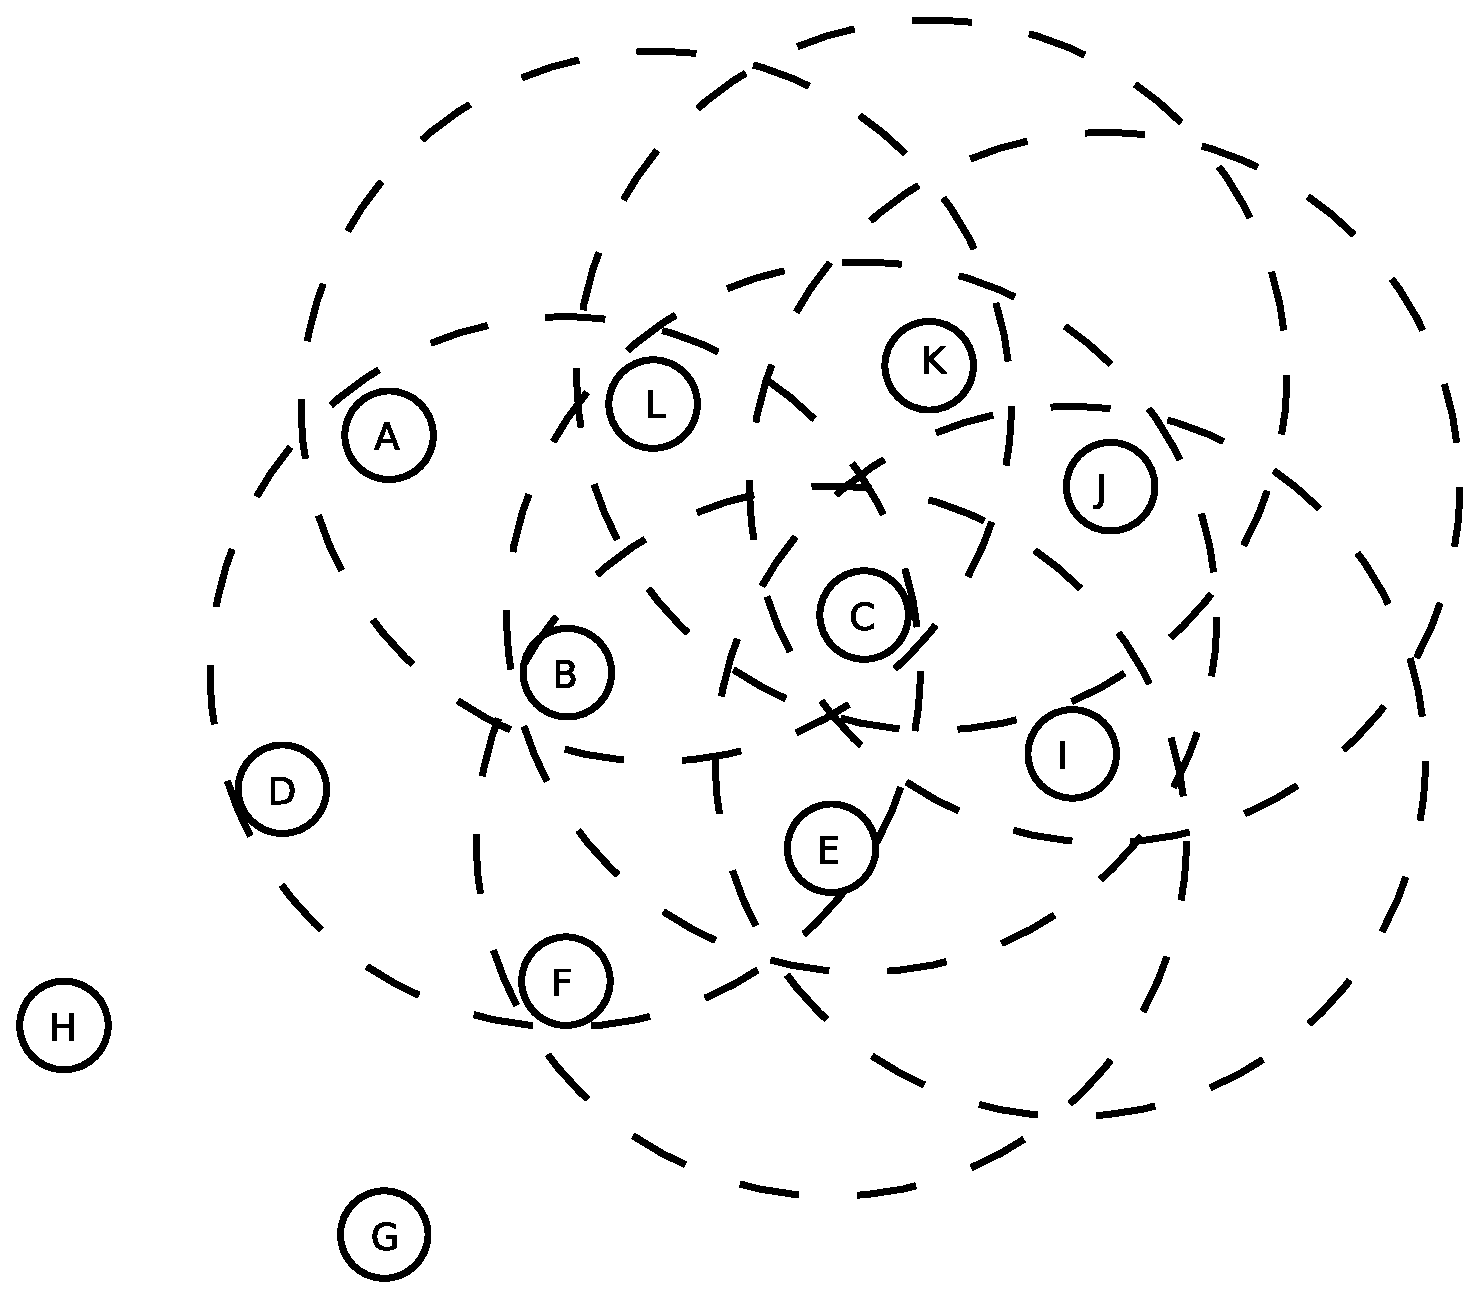
\includegraphics[width=0.7\textwidth]{ejemplonetslots.eps}
 \end{center}
 \caption{Neighbors, and neighbors from neighbors from \ac{AN} C}
 \label{fig:ejemplonetslots}
\end{figure}

In Figure \ref{fig:ejemplonetslots}, a network with 12 \acp{AN} is presented. This \acp{AN} have their coverage painted with the discontinuous line circle,
all \acp{AN} inside a circle are the neighbors from a determinate \ac{AN}. At the same time all this neighbor \acp{AN}, have their own coverage circles.
All \acp{AN} inside this circles and the ones before, cannot transmit at the same time as the first \ac{AN} to avoid hidden terminal problem, the others 
can without risk. In the Figure, \ac{AN} C has as neighbors \acp{AN} B, L, K, J, I and E, and this all have as neighbors the \acp{AN} A, D and F. All this
\acp{AN} cannot transmit at the same time as \ac{AN} C, but \acp{AN} H and G perfectly can.

Thanks to this technique, the bigger the network the more optimal this slots re-use technique, finding that, when \acp{AN} number is not so big this 
technique almost does not help, as all \acp{AN} are inside the neighbor-neighbor distance, but when the \acp{AN} number grows maintaining their 
density, the total needed slots are highly reduced.

To obtain in automatic way the slot distribution among all the \acp{AN} using this technique, the following algorithm is proposed:

\begin{itemize}
 \item First, a matrix with distances between \acp{AN} should be filled, in this matrix the number indicates the distance between
two \acp{AN} in the network. 1 indicates the \acp{AN} are neighbors, 2 indicates that one is neighbor from a neighbor, and so on. For 
the previous network example in Figure \ref{fig:ejemplonetslots}, Table \ref{tab:neighborsmatrix} is extracted.

\begin{table}
 \begin{center}
  \begin{tabular}{c|c|c|c|c|c|c|c|c|c|c|c|c|}
   %\noalign{\vspace*{0.5cm}}
   & \textbf{A} & \textbf{B} & \textbf{C} & \textbf{D} & \textbf{E} & \textbf{F} & \textbf{G} & \textbf{H} & \textbf{I} & 
    \textbf{J} & \textbf{K} & \textbf{L} \\
   \hline
   \textbf{A} & X & 1 & 2 & 1 & 2 & 2 & 2 & 2 & 3 & 3 & 2 & 1 \\
   \hline
   \textbf{B} & 1 & X & 1 & 1 & 1 & 1 & 2 & 2 & 2 & 2 & 2 & 1 \\
   \hline
   \textbf{C} & 2 & 1 & X & 2 & 1 & 2 & 3 & 3 & 1 & 1 & 1 & 1 \\
   \hline
   \textbf{D} & 1 & 1 & 2 & X & 2 & 1 & 1 & 1 & 3 & 3 & 3 & 2 \\
   \hline
   \textbf{E} & 2 & 1 & 1 & 2 & X & 1 & 2 & 3 & 1 & 2 & 2 & 2 \\
   \hline
   \textbf{F} & 2 & 1 & 2 & 1 & 1 & X & 1 & 2 & 2 & 3 & 3 & 2 \\
   \hline
   \textbf{G} & 2 & 2 & 3 & 1 & 2 & 1 & X & 1 & 3 & 4 & 4 & 3 \\
   \hline
   \textbf{H} & 2 & 2 & 3 & 1 & 3 & 2 & 1 & X & 4 & 4 & 4 & 3 \\
   \hline
   \textbf{I} & 3 & 2 & 1 & 3 & 1 & 2 & 3 & 4 & X & 1 & 2 & 2 \\
   \hline
   \textbf{J} & 3 & 2 & 1 & 3 & 2 & 3 & 4 & 4 & 1 & X & 1 & 2 \\
   \hline
   \textbf{K} & 2 & 2 & 1 & 3 & 2 & 3 & 4 & 4 & 2 & 1 & X & 1 \\
   \hline
   \textbf{L} & 1 & 1 & 1 & 2 & 2 & 2 & 3 & 3 & 2 & 2 & 1 & X \\
   \hline
  \end{tabular}
  \caption{\ac{AN} distances matrix}
  \label{tab:neighborsmatrix}
 \end{center}
\end{table}
To fill this matrix, first all the ones have to be filled in (neighbors). Once this is done, all the twos, then all the threes \ldots. For 
example if A - B is 1 and B - C is 1, and A - C was left empty, then A - C will be 2.
 \item After the matrix is completely filled in, it begins slot assignation. First slot is assigned to first row \ac{AN}, in our case A. To 
make it easier, the algorithm will be explained based in the example as it is complicate enough to show all circumstances.
\begin{quote}
 Slot 1 - A
\end{quote}
Then, A row is covered from left to right until a number 3 or bigger is found, then this \ac{AN} gets the same slot as A, in this case I.
\begin{quote}
 Slot 1 - A, I
\end{quote}
Continuing the row, it is found that also J has a number 3, but as I and J have only a 1, they are not compatible and thus J is left out. 
Then, next row is analyzed and B gets a slot.
\begin{quote}
 Slot 1 - A, I \\ Slot 2 - B
\end{quote}
It can be seen that B row has no numbers above 2, this means B cannot share a slot with any other \ac{AN} as it is so close to all of them, 
this makes sense, because as it can be seen in Figure \ref{fig:ejemplonetslots}, B is in the middle of the network. Next row C, gets another
slot and shares it with G but not with H for the same reason as A, I and J.
\begin{quote}
 Slot 1 - A, I \\ Slot 2 - B \\ Slot 3 - C, G
\end{quote}
Next row is D, this \ac{AN} gets its own slot, and covering the row, it is found that I can share the slot with it. But as I was already 
assigned and to allow other \acp{AN} to get also a slot, I is skipped and left for the end. This way, J is the next with number 3 or more 
and that was not assigned yet, so it gets to share slot with J. There is still K with 3 or more, but K and J are not compatible, so K is left out.
We had still I to recheck, in this case it is no more compatible with J and it is hence left out, but if it were compatible with all the 
\acp{AN} in the slot list, then I would get another slot, this would make that an \ac{AN} could get more than one slot if possible, and 
this way idle listening would get reduced.
 \begin{quote}
  Slot 1 - A, I \\ Slot 2 - B \\ Slot 3 - C, G \\ Slot 4 - D, J
 \end{quote}
The matrix analysis continues as described until G row is reached, as G was already assigned, G is skipped and it does not get an extra 
slot like all the \acp{AN} did before. It happens the same with rows H, I, J and K. The current slot assignation is then like follows:
 \begin{quote}
  Slot 1 - A, I \\ Slot 2 - B \\ Slot 3 - C, G \\ Slot 4 - D, J \\ Slot 5 - E, H \\ Slot 6 - F, K
 \end{quote}
Row L. As L did not get a slot before, a new slot is assigned, and covering the row, the first number above 2 found is for G, but
like it was explained before, G has already a slot so is left for the end. H has also a 3 with L, but H was also assigned before and is also 
left for the end.

As the end of the row was reached, and no other \ac{AN} was found to share the slot with L that was not assigned before, the skipped list has
to be checked. In this case the list has more than one element, to assure that all the \acp{AN} get the more slots they can, this list is 
ordered from the \ac{AN} with less slots assigned at the first place to the \ac{AN} with more slots assigned at the last place. This way, it is
avoid for example, that an \ac{AN} gets one slot and other three, when both could take two. In this case both G and H have only one slot 
assigned, that is why any of the two \acp{AN} gets the slot, in this case G was chosen.

This is the final slot distribution:
 \begin{quote}
  Slot 1 - A, I \\ Slot 2 - B \\ Slot 3 - C, G \\ Slot 4 - D, J \\ Slot 5 - E, H \\ Slot 6 - F, K \\ Slot 7 - L, G
 \end{quote}
\end{itemize}

From this example, it can be seen that if \textit{syncPacketsPerSyncPhase} = 3, instead of having $12 \cdot 3 = 36$ slots in every Sync Phase, the slot 
number was reduced to $7 \cdot 3 = 21$ slots, reducing quite a lot listening time in the \acp{MN}.

The word slot was mentioned quite a lot, but how long is an slot?

From Figure \ref{fig:MACFrame} on page~\pageref{fig:MACFrame} and Figure \ref{fig:PPDU} on page~\pageref{fig:PPDU} it is obtained that \ac{MAC}
Layer header has 104 bits. And \ac{PHY} Layer header has 48 bits. If the Application Layer Sync Packet has the following structure:
\begin{itemize}
 \item[-] 8 bit: status
 \item[-] 32 bit: next phase start time-stamp
 \item[-] 16 bit: X dimension from \ac{AN} position
 \item[-] 16 bit: Y dimension from \ac{AN} position
 \item[-] 16 bit: Z dimension from \ac{AN} position
\end{itemize}
Making the \ac{MAC} Layer Payload 88 bits. This together with the 104 bits and the 48 bits, make a total of 240 bits per Sync Packet to be sent.

As it was commented in Chapter \ref{chap:802154standard}: \nameref{chap:802154standard}, the bit rate is 250 Kbits/s. This makes that the Sync
Packet needs 0.96 ms to be transmitted. To this time it has to be added the \ac{CCA} time and the \textit{aTurnaroundTime}. This together with
a security gap in case of bad synchronization, made the slot length 1.5 ms.

To get good results from this technique, a good \acp{AN} distribution is of vital importance. \acp{AN} should be distributed with a density enough
so all \acp{MN} in the network no matter where they are, can reach at least three \acp{AN}, but not so concentrated that all \acp{AN} can
reach each other to allow this technique to reduce the slots number. Whenever a wall or obstacle is found in the network, it could be modeled as
a reduction of the affected \acp{AN} coverage in this direction. 

As all this planning process would be made the first time the network is deployed and probably not changed anymore, the effort will just happen 
at the beginning and will get compensated with a much better network performance that for the random case, this will be proved in Chapter 
\ref{chap:simulationandresults}: \nameref{chap:simulationandresults}.